

\documentclass[DIV=calc, paper=a4, fontsize=10pt]{scrartcl}
\usepackage{makeidx}
\usepackage{graphicx}
\usepackage{flushend}
\usepackage{amssymb}


\usepackage{lmodern}
\usepackage[left=1.5cm,right=1.5cm,top=2.5cm,bottom=2cm]{geometry}
\usepackage{float}		
\bibliographystyle{plain} 
\pagestyle{plain} 
\pagenumbering{arabic}
\usepackage{fancyhdr} 	
\usepackage[T1]{fontenc}
\usepackage[utf8]{inputenc}
\usepackage[spanish]{babel}
\usepackage[spanish,es-tabla]{babel}
\usepackage{hyperref}
\usepackage{graphicx}
\usepackage{siunitx}
\usepackage{lipsum}
\usepackage[protrusion=true,expansion=true]{microtype}
\usepackage{amsmath,amsfonts,amsthm}
\usepackage[svgnames]{xcolor}
\usepackage[svgnames]{xcolor}
\usepackage{booktabs}
\usepackage{fix-cm}
\usepackage{multicol}
\usepackage{url}
\usepackage{cancel}
\usepackage{subfig}
\bibliographystyle{unsrt}

\newenvironment{Figura}
  {\par\medskip\noindent\minipage{\linewidth}}
  {\endminipage\par\medskip}

\usepackage{sectsty}
\allsectionsfont{\usefont{OT1}{phv}{b}{n}}
\usepackage{fancyhdr}
\spanishdecimal{.}
\pagestyle{fancy}
\usepackage{lastpage}
\lhead{}
\chead{}
\rhead{}
\lfoot{}
\cfoot{}
\rfoot{\footnotesize Page \thepage\ of \pageref{LastPage}}
\renewcommand{\headrulewidth}{0.0pt}
\renewcommand{\footrulewidth}{0.4pt}
\usepackage{lettrine}
\newcommand{\initial}[1]{\lettrine[lines=3,lhang=0.3,nindent=0em]{
\color{DarkGoldenrod}{\textsf{#1}}}{}}
\usepackage{titling}
\newcommand{\HorRule}{\color{DarkGoldenrod} \rule{\linewidth}{1pt}}
\pretitle{\vspace{-120pt} \begin{flushleft} \HorRule \fontsize{22}{35} \usefont{OT1}{phv}{b}{n} \color{DarkRed} \selectfont}
\title{Práctica 9. \\ %Aquí va el nombre de la práctica 
Polarización} %Numero de la práctica 
\posttitle{\par
\end{flushleft}
\vskip 0.5em}
\preauthor{\begin{flushleft}\large \lineskip 0.5em \usefont{OT1}{phv}{b}{sl} \color{DarkRed}}
\author{Angel Yair García Pérez \\
Misael Iván Macías Márquez\\
Teodora Irene Ortíz Cruz\\
\small{teodora625@ciencias.unam.mx}\\}
\postauthor{\footnotesize \usefont{OT1}{phv}{m}{sl} \color{Black}
\vspace*{0.1cm} 
Facultad de Ciencias, UNAM
\par\end{flushleft}\HorRule}
\date{27 de Mayo de 2022\\Semestre 2022-2}
\begin{document}
\maketitle
\definecolor{carmine}{rgb}{0.59, 0.0, 0.09}
\begin{abstract}

  \textcolor{carmine}{Resumen:} Usando geometría se calculó el ángulo de Brewster usando como medios al aire y agua, el valor obtenido fue $\theta_{B}= (53.12 \pm 0.04)^{\circ}$, mientras que el valor teórico es $\theta_{B} = 53.123^{\circ}$, comparando ambos resultados se tiene una discrepancia de $0.075<2$ y una incertidumbre $\Delta_{\%}=0.075\%$. Se examinó la polarización de un láser y de un LED con ayuda de un analizador, se encontró que el láser esta polarizado en todas las direcciones mientras que el LED tiene polarización lineal, la polarización está a $60^{\circ}$ del eje horizontal. Por último, usando un polarizador y un analizador se encontró que el coeficiente de atenuación era de $A= (0.9887 \pm 0.0308)$ con una discrepancia de $0.36<2$ y una incertidumbre porcentual de  $\Delta_{\%}=3.11\%$  la intensidad de fuga $B= (0.0015 \pm 0.0011) \frac{W}{m^{2}}$ con una discrepancia de $1.36<2$ y una incertidumbre porcentual de  $\Delta_{\%}=73\%$, debido a las discrepancias se considera que los resultados obtenidos fueron satisfactorios.
  
\end{abstract}
\section*{\textcolor{carmine}{Introducción.}}
El objetivo de este trabajo es analizar la polarización de la luz en distintas situaciones y caracterizar un polarizador\cite{Manual} obteniendo la intensidad de fuga y el coeficiente de atenuación. La importancia de está practica radica en familiarizarse con los distintas maneras de polarizar la luz. Partiendo del marco teórico se espera que el ángulo de Brewster para el agua y aire como medios sea de $53.123^{\circ}$. Se espera que el coeficiente de atenuación del polarizador sea muy cercano a 1 y la intensidad de fuga sea cercana a 0 de tal manera en que se cumpla la Ley de Malus. Para el caso del comportamiento del láser se espera encontrar que este esta polarizado en todas las direcciones mientras que para la luz LED se espera una polarización lineal a un ángulo de $60^{\circ}$ del eje horizontal. 
\subsection*{\textcolor{carmine}{Polarización}}
La luz se puede tratar como una onda electromagnética por lo que se le puede asociar una polarización la cual es una propiedad de las ondas que pueden oscilar con más de una orientación. Existen dos tipos de polarizaciones principales conocidas como lineal, cuando  la orientación del campo eléctrico es constante aunque su magnitud y signo varían con el tiempo y la circular que aparece cuando ambas ondas constitutivas tienen igual amplitud\cite{book}.
\subsection*{\textcolor{carmine}{Polarización por reflexión}}
Una forma de polarizar la luz es por medio de la reflexión, supongamos que un rayo incide en algún medio y sale reflejado dado que la luz que tiene un campo eléctrico paralelo al plano de incidencia, el coeficiente de reflexión baja a cero a un determinado ángulo entre 0º y 90° y la luz reflejada en ese ángulo, está polarizada linealmente, con sus vectores de campo eléctrico perpendicular al plano de incidencia y paralelo al plano de la superficie donde se refleja\cite{book}. Para otros ángulos, se polarizada parcialmente. El ángulo en que esto ocurre se llama ángulo de polarización o ángulo de Brewster y aplicando ley de Snell para las condiciones del problema $\theta_{1}+\theta_{2}=90^{\circ} $se tiene que\cite{pagina}
\begin{equation}
    \theta_{B}=\tan^{-1}\left(\frac{n_{2}}{n_{1}}\right)
\end{equation}
\begin{figure}[H]
    \centering
    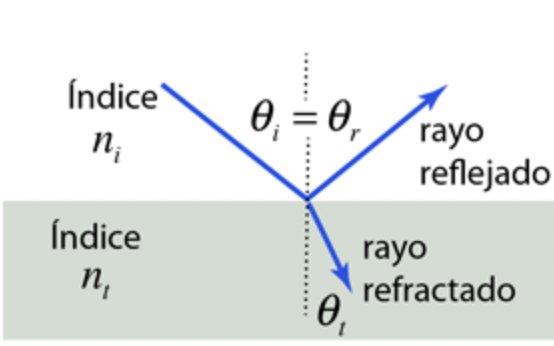
\includegraphics[width=5cm]{Introducción/Captura de Pantalla 2022-05-22 a la(s) 14.21.18.png}
    \caption{Se observa el rayo incidente desde un medio $n_{i}=n_{1}$ a un medio $n_{t}=n_{2}$ con la condición $\theta_{1}+\theta_{2}=90^{\circ}$ y por medio de ley de Snell da el ángulo de Brewster\cite{pagina}.}
    \label{fig:my_label}
\end{figure}
\subsection*{\textcolor{carmine}{Ley de Malus y Dicroísmo}}
En su acepción más amplia el término dicroísmo se refiere a la
absorción selectiva de una de las componentes del estado polarizado, el dicroísmo ocurre cuando se coloca un polarizador y un analizador en serie con sus ejes de trasmisión paralelos entonces la luz polarizada linealmente pasará por el primer polarizador pero no sera absorbida por el analizador\cite{book}. Si ahora se considera que la luz incide con un ángulo $\beta$  con una irradiancia $I_{0}=\frac{c\varepsilon^{2}}{2}E_{0}^{2}$ y una polarización lineal al analizador con eje de transmisión en un ángulo $\theta$
se puede construir la matriz asociada a la polarización y con ella la irradiancia que llega al detector será dada por la Ley de Malus\cite{Manual}.
\begin{equation}
    I=I_{0}\cos^{2}(\theta-\beta)
\end{equation}
Sin embargo a la hora de llevar acabo experimentos se ha detectado que si se coloca un polarizador ortogonal al eje de transmisión la intensidad de salida no es cero a ese valor se le llama intensidad de fuga, si el polarizador es paralelo a la polarización de entrada aparecerá un coeficiente de atenuación provocando que la intensidad de salida sea menor a la de entrada y entonces la ley de Malus se reescribe como
\begin{equation}
    I=A(I_{0}\cos^{2}(\theta-\beta))+B
\end{equation}
\begin{figure}[H]
    \centering
    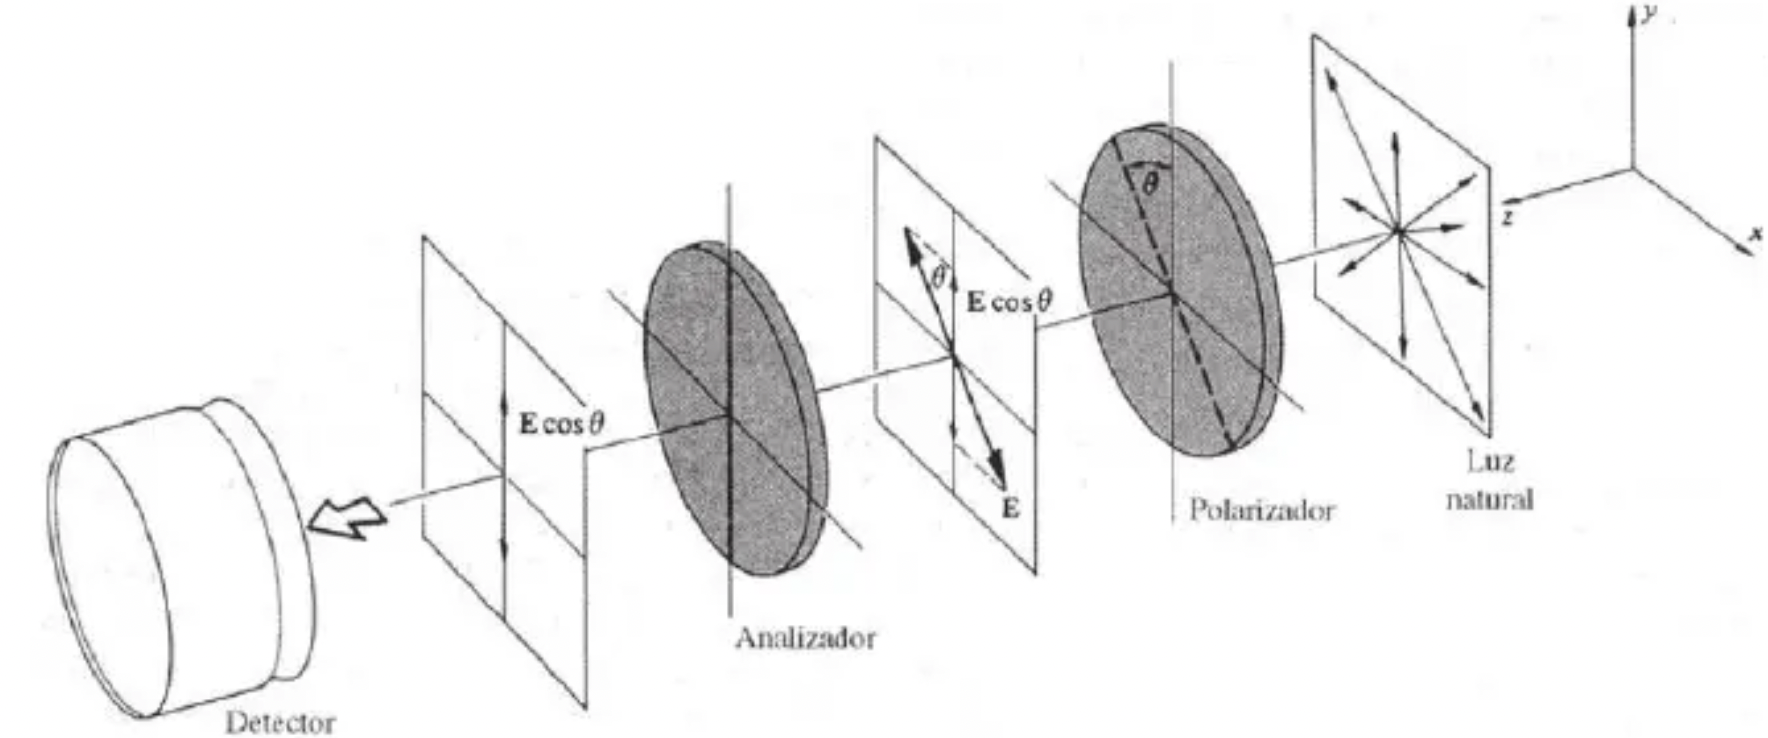
\includegraphics[width=7cm]{Introducción/Captura de Pantalla 2022-05-22 a la(s) 14.30.46.png}
    \caption{Se observa una fuente de luz que incide en un analizador y luego la luz que pasa llega a un polarizador ubicado a un ángulo $\theta$ con respecto a la vertical\cite{book}.}
    \label{fig:my_label}
\end{figure}
\section*{\textcolor{carmine}{Desarrollo Experimental.}}
\subsection*{\textcolor{carmine}{Polarización por Reflexión}}
Para este método se colocó un recipiente largo con agua y una luz LED blanca frente al recipiente para que produjera un reflejo como se muestra en la Figura 3, luego un integrante del equipo de trabajo se colocó a una distancia mayor a un metro con un polarizador, con el polarizador en mano se buscó la posición en donde el reflejo presento menor intensidad. Con una cinta métrica se midió la distancia del reflejo hasta el punto donde estaba parado el individuo con el polarizador y luego se tomó la medida de los pies hasta los ojos. Se repitió el experimento para cada uno de los integrantes y se registraron los datos con una incertidumbre de apreciación $\sigma_{ap}=\pm\hspace{0.1cm}0.05\hspace{0.1cm}\text{cm}$ dada por la mínima escala entre 2 de la cinta métrica 
\begin{figure}[H]
    \centering
    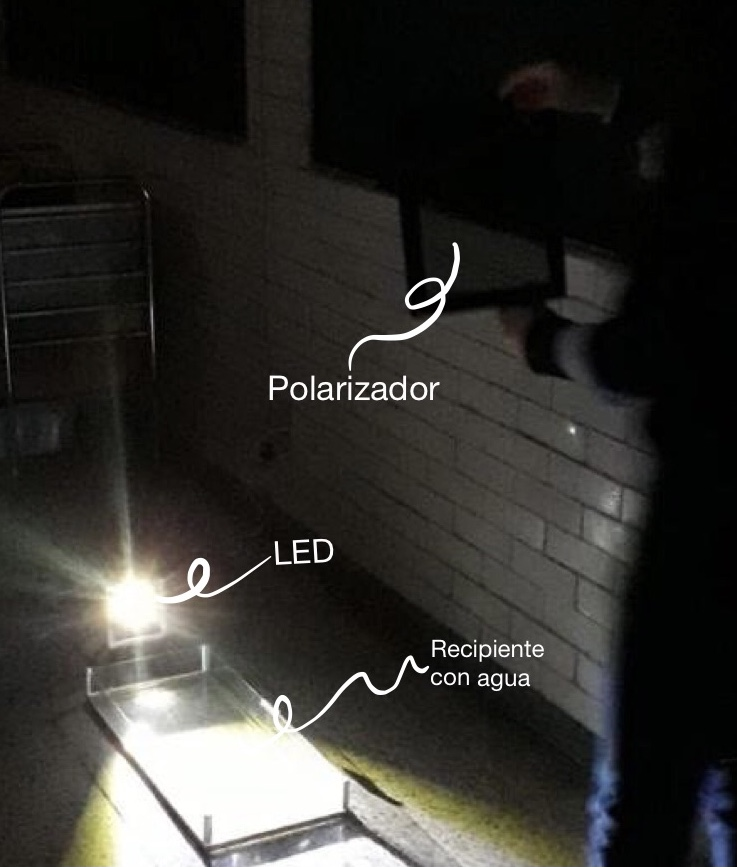
\includegraphics[width=5cm]{Introducción/9B226505-C76F-45D1-84D8-0F126BD8B16B.jpeg}
    \caption{\textbf{Polarización por reflexión.} Se observa el arreglo experimental empleado para observar la polarización por reflexión.}
    \label{fig:my_label}
\end{figure}
\subsection*{\textcolor{carmine}{Polarización por una fuente de luz}}

\textcolor{carmine}{\textbf{Polarización de un Láser.}}\\
En la mesa óptica se se coloco un láser, un polarizador con escala de ángulos y frente a el se colocó un radiómetro como se muestra en la Figura 4(a) y por último se rodeó el arreglo experimental con tablas negras. Se midió la irradiancia que había sin que el láser estuviera encendido dando un valor de $0.839\frac{mW}{m^2}$ y luego se encendió el láser. Para esta parte se fue girando el analizador cada $10^{\circ}$ y se registro una incertidumbre de apreciación para los ángulos $\sigma_{ap}=\pm\hspace{0.1cm}0.5^{\circ}$. En cada ángulo se registró la irradiancia medida por el radiómetro con la incertidumbre dada por el mismo aparato la cual solía tomar los valores de  $\sigma_{ap}=\pm\hspace{0.1cm}0.05\hspace{0.1cm}\frac{W}{m^{2}}$, $\sigma_{ap}=\pm\hspace{0.1cm}1.01\hspace{0.1cm}\frac{mW}{m^{2}}$  y 
$\sigma_{ap}=\pm\hspace{0.1cm}0.01\hspace{0.1cm}\frac{W}{m^{2}}$\\

\textcolor{carmine}{\textbf{Polarización de un LED.}}\\
En la mesa óptica se se coloco un LED, un polarizador con escala de ángulos y frente a el se colocó un radiómetro como se muestra en la Figura 4(b) y por último se rodeó el arreglo experimental con tablas negras. Se midió la irradiancia que había sin que el LED estuviera encendido dando un valor de $0.839\frac{mW}{m^2}$ y luego se encendió el LED. Para esta parte se fue girando el analizador cada $10^{\circ}$ y se registro una incertidumbre de apreciación para los ángulos $\sigma_{ap}=\pm\hspace{0.1cm}0.5^{\circ}$. En cada ángulo se registró la irradiancia medida por el radiómetro con la incertidumbre dada por el mismo aparato la cual solía tomar los valores de  $\sigma_{ap}=\pm\hspace{0.1cm}0.05\hspace{0.1cm}\frac{W}{m^{2}}$, $\sigma_{ap}=\pm\hspace{0.1cm}1.01\hspace{0.1cm}\frac{mW}{m^{2}}$ y  
$\sigma_{ap}=\pm\hspace{0.1cm}0.01\hspace{0.1cm}\frac{W}{m^{2}}$
\begin{figure}[H]
 \centering
  \subfloat[Polarización de un láser]{
   \label{f:gato}
    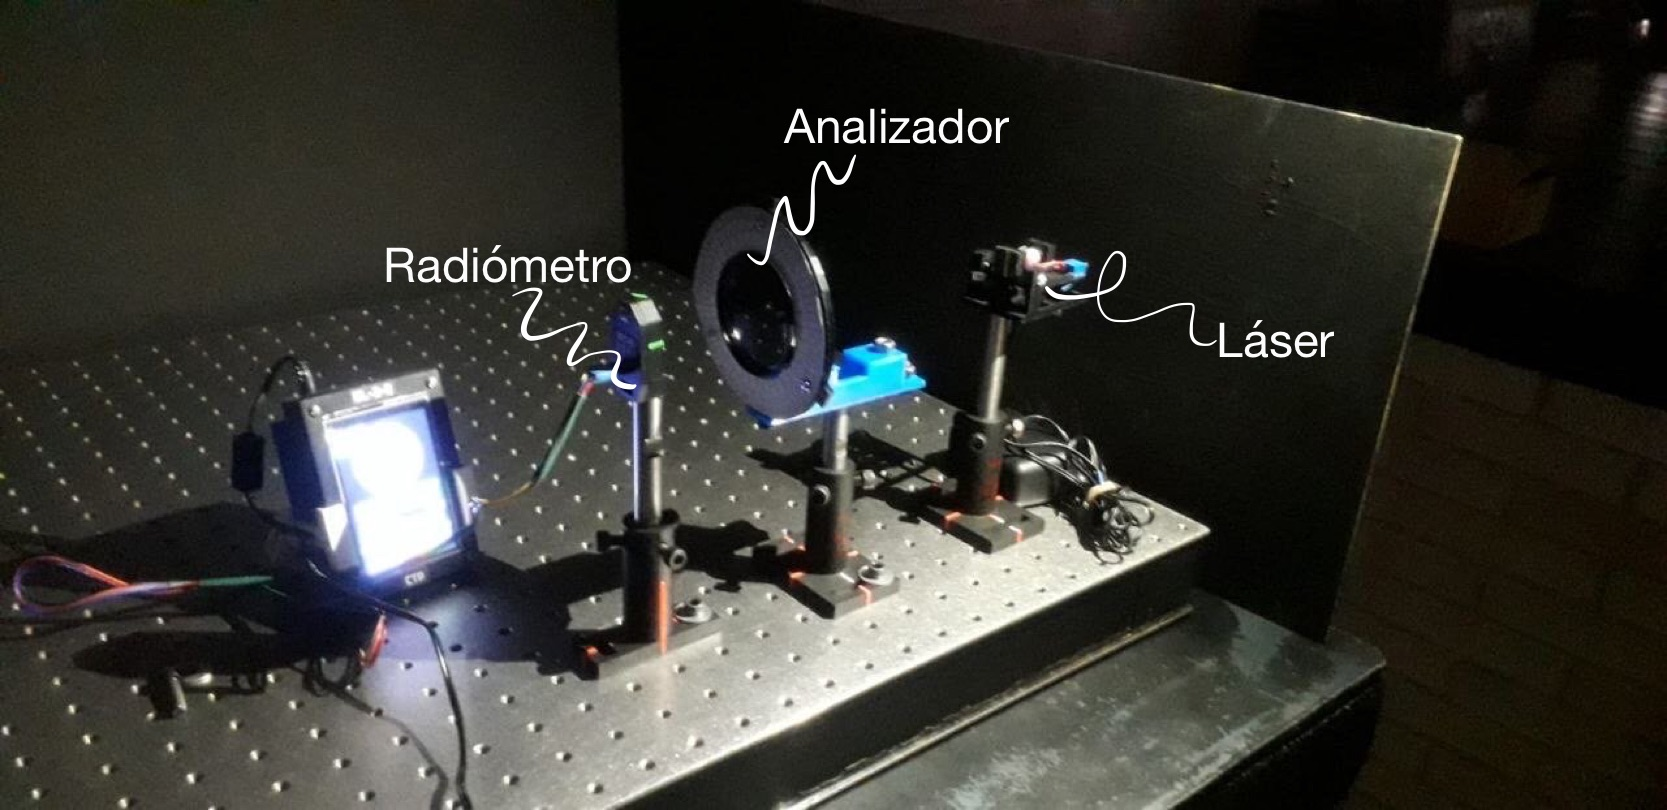
\includegraphics[width=0.4\textwidth]{Introducción/DA2EC464-1882-42B3-A65F-15308975BB5D.jpeg}}
  \subfloat[Polarización de una luz LED]{
   \label{f:tigre}
    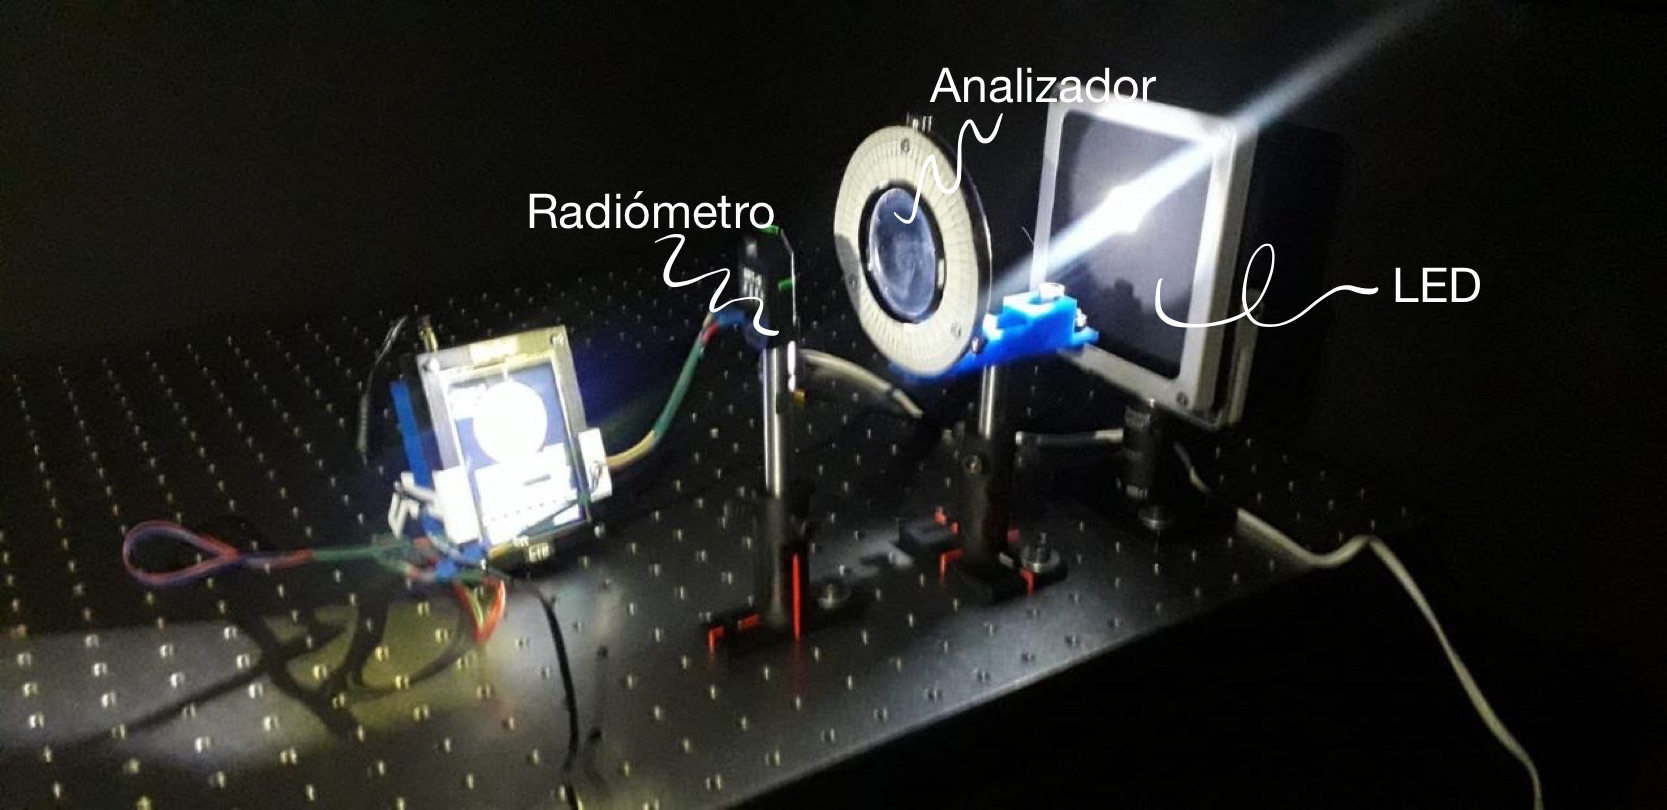
\includegraphics[width=0.4\textwidth]{Introducción/15925101-1223-498E-8AC3-5E0AD42F9ED4.jpeg}}
 \caption{4(a) se observa el arreglo experimental utilizado para estudiar la polarización de una luz láser. 4(b) se observa el arreglo experimental utilizado para estudiar la polarización de una luz LED}
 \label{f:animales}
\end{figure}
\subsection*{\textcolor{carmine}{Dicroísmo(Ley de Malus)}}
Para esta parte con al mismo arreglo de la parte experimental anterior y se fijo el polarizador a un ángulo $\beta=(50\pm\hspace{0.1cm}0.5)^{\circ}$. Con el radiómetro se midió una intensidad $I_{0}=(0.1386\pm\hspace{0.1cm}0.00005)\hspace{0.1cm}\frac{W}{m^{2}}$. Luego  entre el polarizador y el foto-detector se colocó un analizador, como se muestra en la Figura 5, con escala de ángulos la cual tenia una incertidumbre de apreciación de $\sigma_{ap}=\pm\hspace{0.1cm}0.5^{\circ}$. Partiendo de $0^{\circ}$ el analizador se fue girando cada $10^{\circ}$ hasta llegar a $360^{\circ}$ y se registraron las medidas de irradiancia dadas por el radiómetro en cada ángulo, con la incertidumbre dada por el mismo aparato la cual solía tomar los valores de  $\sigma_{ap}=\pm\hspace{0.1cm}0.05\hspace{0.1cm}\frac{W}{m^{2}}$, $\sigma_{ap}=\pm\hspace{0.1cm}1.01\hspace{0.1cm}\frac{mW}{m^{2}}$ y  
$\sigma_{ap}=\pm\hspace{0.1cm}0.01\hspace{0.1cm}\frac{W}{m^{2}}$. 
Luego se cambió el ángulo del polarizador por $\beta=(100\pm\hspace{0.1cm}0.5)^{\circ}$ e intensidad $I_{0}= (0.0308\pm\hspace{0.1cm}0.00005)\hspace{0.1cm}\frac{W}{m^{2}}$ y  se registraron las medidas de irradiancia dadas por el radiómetro en cada ángulo, con las incertidumbres ya conocidas, $\sigma_{ap}=\pm\hspace{0.1cm}0.05\hspace{0.1cm}\frac{W}{m^{2}}$, $\sigma_{ap}=\pm\hspace{0.1cm}1.01\hspace{0.1cm}\frac{mW}{m^{2}}$ y  
$\sigma_{ap}=\pm\hspace{0.1cm}0.01\hspace{0.1cm}\frac{W}{m^{2}}$. 
\begin{figure}[H]
    \centering
    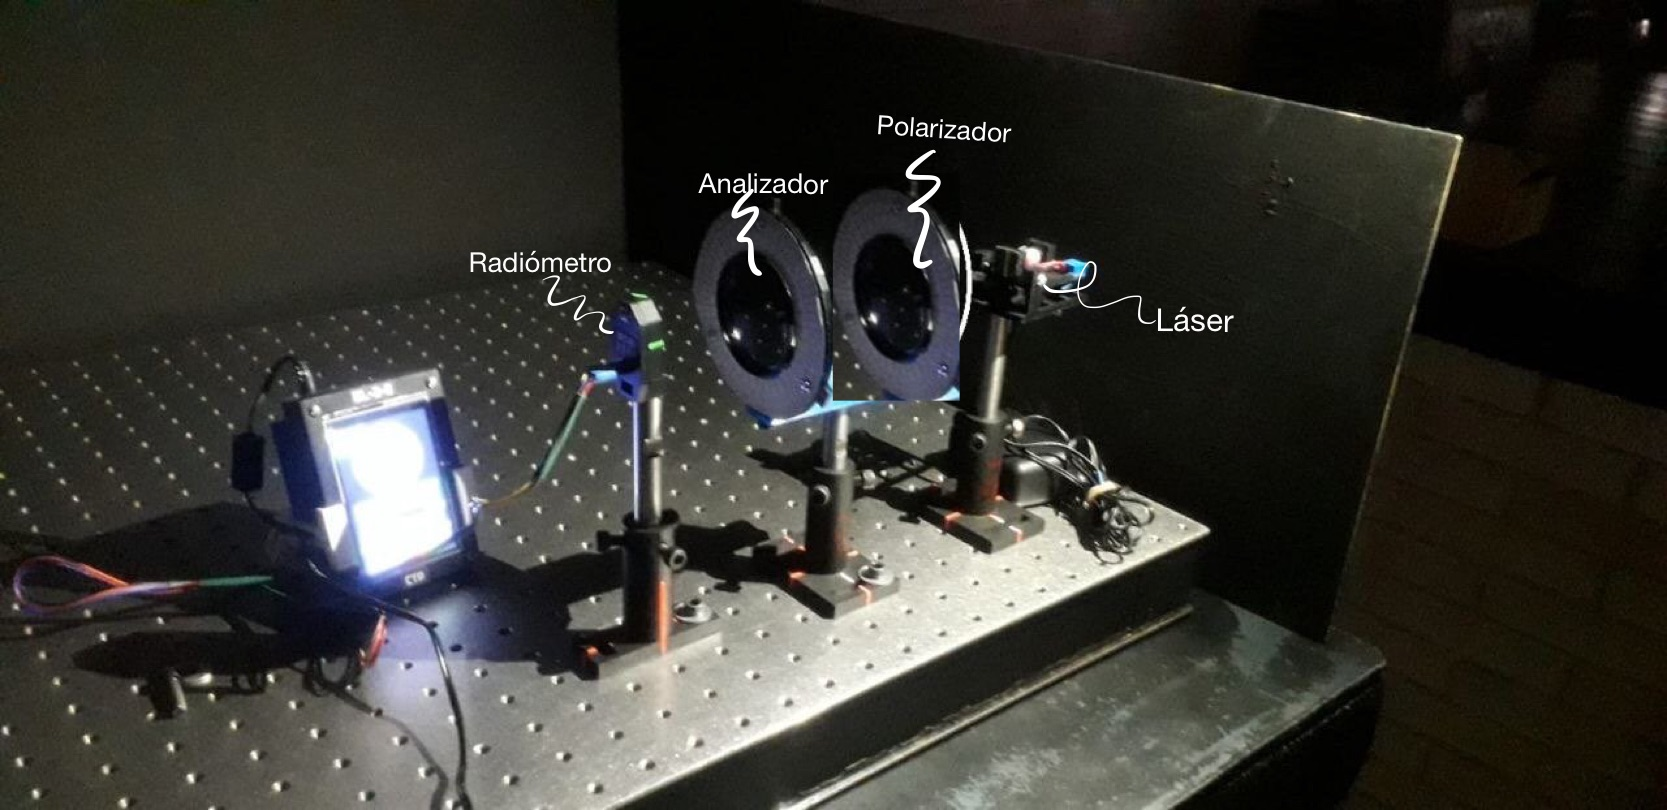
\includegraphics[width=6.5cm]{Introducción/8995BA78-DB6F-45EB-9518-A1A5FA02F795.jpeg}
    \caption{Arreglo experimental utilizado para probar la Ley de Malus. En el se observa un analizador seguido de un polarizador al que se le incide luz láser}
    \label{fig:my_label}
\end{figure}
\section*{\textcolor{carmine}{Resultados y Análisis.}}

\subsection*{\textcolor{carmine}{Polarización por reflexión}}

De la geometría sabemos que:

\begin{equation*}
    \theta = \tan^{-1}{\left(\frac{y}{x}\right)}
\end{equation*}

Propagando su incertidumbre:

\begin{equation*}
    \Delta \theta = \sqrt{\left(\frac{\partial \theta}{\partial y}\Delta y\right)^{2}+ \left(\frac{\partial \theta}{\partial x} \Delta x\right)^{2}}
\end{equation*}

\begin{equation*}
    = \csc^{2}{\left(\frac{y}{x}\right)}\sqrt{\left(\frac{\Delta y}{x}\right)^{2} + \left(\frac{y \Delta x}{x^{2}}\right)^{2}}
\end{equation*}

La relación entre $\theta_{B}$ y $\theta$ con su incertidumbre es:

\begin{equation*}
    \theta_{B} = 90^{\circ}-\theta \hspace{1cm} \Delta \theta_{B} = \Delta \theta
\end{equation*}

\begin{figure}[H]
    \centering
    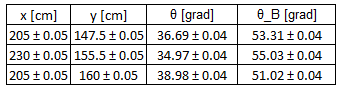
\includegraphics{tablas/tabla 1.PNG}
    \caption{Tabla de alturas y distancias medidas con sus correspondientes ángulos.}
    \label{fig:my_label}
\end{figure}

Promediando los valores de $\theta_{B}$:

\begin{equation*}
    \theta_{B}= (53.12 \pm 0.04)^{\circ}
\end{equation*}

Sustituyendo $n_{\text{agua}} = 1.333 $ y $n_{\text{aire}} = 1$ en la ecuación (1) se obtiene un valor teórico de:

\begin{equation*}
    \theta_{B} = \tg^{-1}{\left(\frac{n_{\text{agua}}}{n_{\text{aire}}}\right)} = \tg^{-1}(1.33) = 53.123^{\circ}
\end{equation*}

\subsection*{\textcolor{carmine}{Polarización de una fuente de luz}}

\begin{figure}[H]
    \centering
    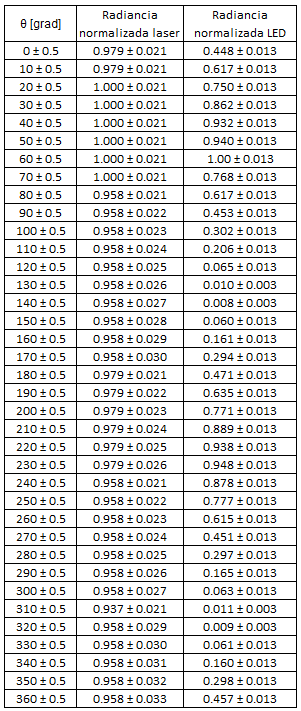
\includegraphics[scale=0.75]{tablas/tabla 2.PNG}
    \caption{Tabla de Radiancias normalizadas del LED y láser vs ángulos $\theta$.}
    \label{fig:my_label}
\end{figure}

\begin{figure}[H]
    \centering
    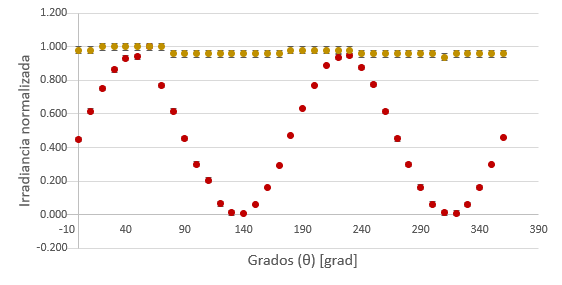
\includegraphics{graficas/grafica 1.PNG}
    \caption{Gráfica de Radiancia normalizada del LED y láser vs ángulos $\theta$.}
    \label{fig:my_label}
\end{figure}

%láser no linealmente polarizada (?)
%LED linealmente polarizada  (?)
De la figura $6$ podemos deducir que el láser no esta linealmente polarizado y que el LED esta linealmente polarizado, el láser tiene una polarización en todos los sentidos porque al cambiar el ángulo del eje de transmisión del analizador la radiancia del láser es prácticamente constante, la fuente LED tiene una polarización lineal, esto se puede ver en la figura porque al cambiar el ángulo del eje de transmisión del analizador la radiancia de esta toma máximos y mínimos cada $180^{\circ}$, la polarización esta dada por el primer ángulo del valor máximo, este ángulo es $60^{\circ}$, por lo tanto la polarización esta a $60^{\circ}$ del eje horizontal.

\subsection*{\textcolor{carmine}{Dicroísmo (Ley de Malus)}}

La ley de Malus nos dice que:

\begin{equation*}
    x = I_{0} \cos^{2} (\theta - \beta)
\end{equation*}

Propagando su incertidumbre:

\begin{equation*}
    \Delta x = 4 \sin^{2}{(\theta  - \beta)} \cos^{2}{(\theta - \beta)}\sqrt{(\Delta \theta)^2 + (\Delta  \beta)^2}
\end{equation*}

\begin{figure}[H]
 \centering
  \subfloat[$\beta = 100^{\circ}$]{
   \label{f:gato}
    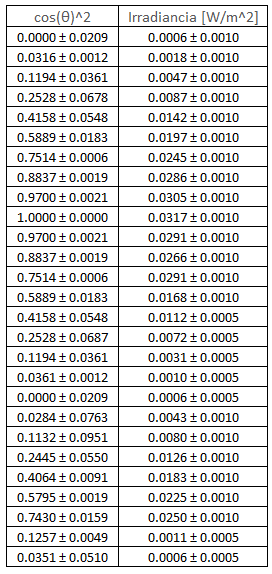
\includegraphics[width=0.35\textwidth]{tablas/tabla 100.PNG}}
  \subfloat[$\beta = 50^{\circ}$]{
   \label{f:tigre}
    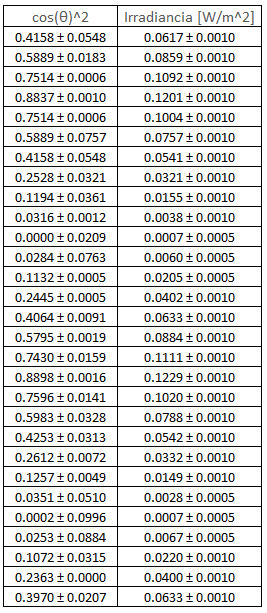
\includegraphics[width=0.35\textwidth]{tablas/tabla 50.PNG}}
 \caption{Tablas de coseno cuadrado de $\theta - \beta$ e Irradiancia.}
 \label{f:animales}
\end{figure}

\begin{figure}[H]
 \centering
  \subfloat[$\beta = 100^{\circ}$]{
   \label{f:gato}
    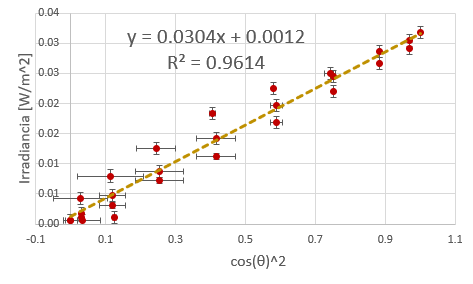
\includegraphics[width=0.5\textwidth]{graficas/grafica beta 100.PNG}}
  \subfloat[$\beta = 50^{\circ}$]{
   \label{f:tigre}
    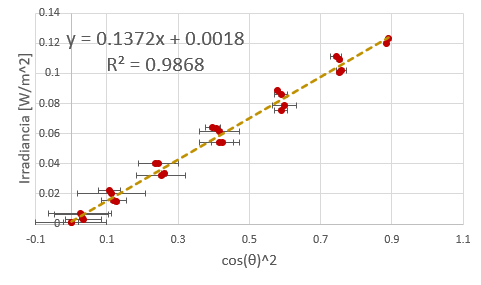
\includegraphics[width=0.5\textwidth]{graficas/grafica beta 50.PNG}}
 \caption{Gráficas de coseno cuadrado de $\theta - \beta$ e Irradiancia.}
 \label{f:animales}
\end{figure}

Se espera algo de la forma:

\begin{equation*}
    I = A x + B
\end{equation*}

Donde $A$ es el coeficiente de atenuación:

\begin{equation*}
    A = \frac{m}{I_0} \hspace{1cm} \Delta A = \sqrt{\left(\frac{\Delta m}{I_{0}}\right)^{2} + \left(\frac{m\Delta I_0}{I_{0}^{2}}\right)^2}
\end{equation*}
Y $B$ la intensidad de fuga:
\begin{equation*}
    B=b \hspace{1cm} \Delta B = \Delta b
\end{equation*}

Despues de hacer el ajuste, con el metodo de minimos cuadrados, se promedio y se obtuvo que:

\begin{equation*}
    A= (0.9887 \pm 0.0308) \hspace{1cm} B= (0.0015 \pm 0.0011) \frac{W}{m^{2}}
\end{equation*}


\section*{\textcolor{carmine}{Discusión y Conclusión.}}

Se obtuvo que el angulo de Brewster es:
\begin{equation*}
    \theta_{B}= (53.12 \pm 0.04)^{\circ}
\end{equation*}
Comparando con el valor teorico:
\begin{equation*}
    \theta_{B} = 53.123^{\circ}
\end{equation*}
Podemos ver el resultado es bueno.
\\\\
El laser tiene una polarizacion en todos los sentidos, ya que si este paso por un analizador, al cambiar el eje de transmision el valor de la radiancia del laser siempre sera constante, mientras que el LED tiene una polarizacion lineal ya que la radiancia toma valores maximos y minimos cada $180^{\circ}$, la polarizacion del LED esta a $60^{\circ}$ del eje horizontal.
\\
Para la ley de Malus:

\begin{equation*}
    I = A (I_{0}\cos^2{\theta - \beta} ) + B
\end{equation*}

Se encontró que el coeficiente de atenuación es de $A= (0.9887 \pm 0.0308)$ y que la intensidad de fuga es $B= (0.0015 \pm 0.0011) \frac{W}{m^{2}}$
\nocite{*}

\bibliography{biblio}

\end{document}